%%%%%%%%%% Page 1 - Col 1 %%%%%%%%%%
\newpage
\colorfulheader{cuda programming}

\begin{minipage}[t]{0.485\textwidth}
    CUDA: Parallel computing platform developed by NVIDIA. Stands for \textbf{C}ompute \textbf{U}nified \textbf{D}evice \textbf{A}rchitecture.\\

    Before going into GPU, there are 5 steps for an instruction to finish (CPU-wise): (1) Fetch, (2) Decode, (3) Execute, (4) Memory Access, and (5) Register Write-Back. These steps are the five-stage for an \textbf{RISC} architecture.\\

    One way of doing work in parallel is via \textbf{Instruction Level Parallelism} where in one clock cycle (of the CPU) many steps of different instructions are executed in parallel.\\

    A CPU has a larger instruction set than a GPU, a complex ALU, a better branch prediction logic, and a more sophisticated caching/pipeline schemes. Instruction cycles are also faster.\\

    The GPU comprises many cores processor and each core runs at a clock speed slower than a CPU's clock. GPU focus on execute throughput in parallel. For example, the GTX 280 GPU has 240 cores, each one multi-threaded, and with a SIMD (Single Instruction Multiple Data) paradigm, each core shares its control and instruction cache with the other seven cores.\\

    Sequential programs do not have a \quotes{working set} of data, and most of its data can be stored in \textbf{L1}, \textbf{L2}, or \textbf{L3} cache, who are faster to fetch than from RAM.\\

    Types of memories
    \begin{itemize}
        \setlength\itemsep{1pt}
        \item \textbf{DRAM} or Dynamic RAM. Slowest but least expensive (money-wise?).
        \item \textbf{SRAM} or Static RAM. Faster and does not require constant refreshing as DRAM. It is also known as \textbf{Cache Memory}. SRAM being expensive a processor would have few caches, for example, the Intel 486 microprocessor has only 8KB of SRAM.
        \item \textbf{VRAM} or Video RAM. Similar to DRAM but can be written-to and read-from simultaneously. An example usage is reading from VRAM and sending it directly to the screen without having to wait for the CPU to write into global memory.
    \end{itemize}

    The structure of a CUDA code has a GPU (device) part and a CPU (host) part. The host part is compiled by a traditional C compiler (like GCC), the device code requires a compiler that understands the special keywords used, an example of such compiler would be NVCC (NVIDIA C Compiler). When parsing the code, to differentiate what is host or device, NVCC looks for specific keywords, for example \texttt{\_\_device\_\_} or \texttt{kernel\_name<<<>>>}.\\

    Programmer has \textbf{explicit} control over the number of threads to be launched.
    \begin{equation*}
        \text{threads} \xrightarrow{\text{packed into}} \text{blocks} \xrightarrow{\text{packed into}} \text{grids}
    \end{equation*}
\end{minipage}
%%%%%%%%%%%%%%%%%%%%%%%%%%%%%%%%%%%%
\hspace{10pt}
%%%%%%%%%% Page 1 - Col 2 %%%%%%%%%%
\begin{minipage}[t]{0.485\textwidth}
    To execute a kernel on the GPU the usual pipeline is
    \begin{enumerate}
        \setlength\itemsep{0pt}
        \item Allocate memory on device \parenthesis{\texttt{cudaMalloc()}}
        \item Transfer data from host memory into device memory \parenthesis{\texttt{cudaMemcpy()}}
        \item Execute kernel \\ \parenthesis{\texttt{kernel<<<blocksPerGrid,threadsPerBlock>>>()}}
        \item Transfer data from device memory into host memory \parenthesis{\texttt{cudaMemcpy()}}
        \item Release memory on device \parenthesis{\texttt{cudaFree()}}
    \end{enumerate}
    \begin{customcenter}[0pt]
        \begin{tabular}{|c|c|c|}
        \hline
        & \textbf{Executed on} & \textbf{Callable from} \\
        \hline
        \texttt{\_\_device\_\_} & GPU & CPU \\
        \hline
        \texttt{\_\_global\_\_} & CPU & GPU \\
        \hline
        \texttt{\_\_host\_\_} & GPU & GPU \\
        \hline
        \end{tabular}
    \end{customcenter}
    \vspace{8pt}
    Inside a kernel, important keywords to obtain indices are \textbf{gridDim}, \textbf{blockDim}, \textbf{blockIdx}, and \textbf{threadIdx}. Each one has 3 components \texttt{[x, y, z]}. For example, if we want to apply a kernel to an image of dimensions \parenthesis{76 $\times$ 62} we could launch 5120 = (80 $\times$ 64), which is a multiple of 4, threads and each block having 256 = (16 $\times$ 16) of them. Thus, a way of specifying the kernel is
    \begin{lstlisting}
        dim3 threadsPerBlock(16,16,1)
        dim3 blocksPerGrid(5,4,1)
        kernel<<<blocksPerGrid,threadsPerBlock>>()
        __device__ kernel() 
        {
            int row = blockIdx.x * blockDim.x + threadIdx.x;
            int col = blockIdx.y * blockDim.y + threadIdx.y;
            ... remaining code ...
        }
    \end{lstlisting}
    \vspace{5pt}
    Execution resources assigned to threads per block are organized in \textbf{Streaming Multiprocessors} (SM). Multiple blocks of threads can be assigned to a single SM. After assigning to a SM, the block is divided into sets of 32 threads (called \textbf{warp}).\\

    CUDA API has the built-in method \texttt{\_\_syncthreads()} that causes all threads in a blocked to be blocked at the calling location until each thread reaches that point. This is to ensure \textbf{phase synchronization} when used.
    \begin{customcenter}[5pt]
        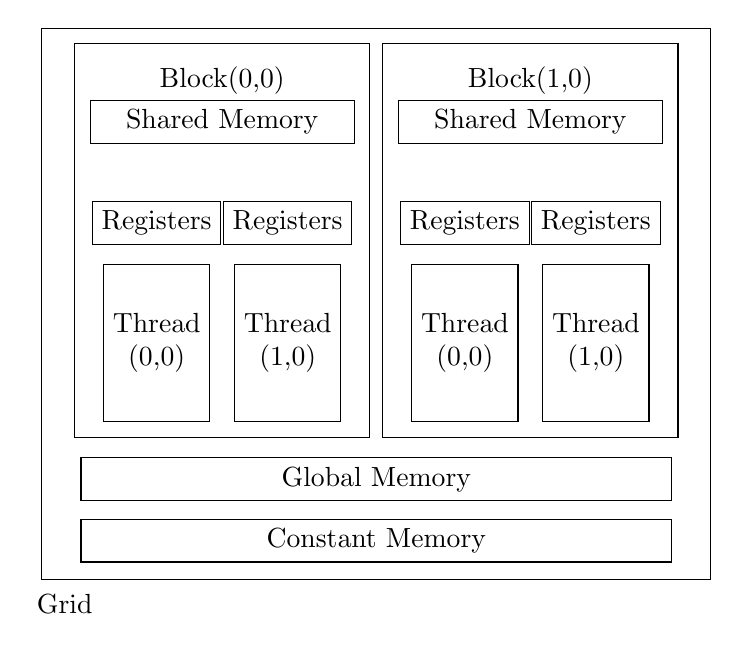
\begin{tikzpicture}
            \node[rectangle,draw,minimum width=8.5cm,minimum height=7cm] (node1) at (0,0) {};
            \node[yshift=-0.3cm,xshift=0.3cm] (node0) at (node1.south west) {Grid};
            \node[rectangle,draw,minimum width=7.5cm,yshift=0.5cm] (node2) at (node1.south) {Constant Memory};
            \node[rectangle,draw,minimum width=7.5cm,yshift=0.5cm] (node3) at (node2.north) {Global Memory};
            % Grid (0,0)
            \node[rectangle,draw,minimum height=5cm,yshift=2.75cm,minimum width=3.75cm,xshift=+1.8cm] (node4) at (node3.north west) {};
            \node[rectangle,draw,minimum width=3.35cm,yshift=-1cm] (node6) at (node4.north) {Shared Memory};
            \node[rectangle,draw,minimum width=1.5cm,yshift=-1cm,xshift=+0.85cm] (node7) at (node6.south west) {Registers};
            \node[rectangle,draw,minimum width=1.5cm,yshift=-1cm,xshift=-0.85cm] (node8) at (node6.south east) {Registers};
            \node[rectangle,draw,minimum height=2cm,align=center,yshift=-1.25cm] (node9) at (node7.south) {Thread \\ (0,0)};
            \node[rectangle,draw,minimum height=2cm,align=center,yshift=-1.25cm] (node10) at (node8.south) {Thread \\ (1,0)};
            \node[yshift=0.25cm] (node11) at (node6.north){Block(0,0)};
            % Grid (1,0)
            \node[rectangle,draw,minimum height=5cm,yshift=2.75cm,minimum width=3.75cm,xshift=-1.8cm] (node5) at (node3.north east) {};
            \node[rectangle,draw,minimum width=3.35cm,yshift=-1cm] (node14) at (node5.north) {Shared Memory};
            \node[rectangle,draw,minimum width=1.5cm,yshift=-1cm,xshift=+0.85cm] (node15) at (node14.south west) {Registers};
            \node[rectangle,draw,minimum width=1.5cm,yshift=-1cm,xshift=-0.85cm] (node16) at (node14.south east) {Registers};
            \node[rectangle,draw,minimum height=2cm,align=center,yshift=-1.25cm] (node17) at (node15.south) {Thread \\ (0,0)};
            \node[rectangle,draw,minimum height=2cm,align=center,yshift=-1.25cm] (node18) at (node16.south) {Thread \\ (1,0)};
            \node[yshift=0.25cm] (node19) at (node14.north){Block(1,0)};
        \end{tikzpicture}
    \end{customcenter}
\end{minipage}
%%%%%%%%%%%%%%%%%%%%%%%%%%%%%%%%%%%%